\documentclass[12pt,letterpaper]{article}
\usepackage{graphicx,textcomp}
\usepackage{natbib}
\usepackage{setspace}
\usepackage{fullpage}
\usepackage{color}
\usepackage[reqno]{amsmath}
\usepackage{amsthm}
\usepackage{fancyvrb}
\usepackage{amssymb,enumerate}
\usepackage[all]{xy}
\usepackage{endnotes}
\usepackage{lscape}
\newtheorem{com}{Comment}
\usepackage{float}
\usepackage{hyperref}
\newtheorem{lem} {Lemma}
\newtheorem{prop}{Proposition}
\newtheorem{thm}{Theorem}
\newtheorem{defn}{Definition}
\newtheorem{cor}{Corollary}
\newtheorem{obs}{Observation}
\usepackage[compact]{titlesec}
\usepackage{dcolumn}
\usepackage{tikz}
\usetikzlibrary{arrows}
\usepackage{multirow}
\usepackage{xcolor}
\newcolumntype{.}{D{.}{.}{-1}}
\newcolumntype{d}[1]{D{.}{.}{#1}}
\definecolor{light-gray}{gray}{0.65}
\usepackage{url}
\usepackage{listings}
\usepackage{color}
\definecolor{codegreen}{rgb}{0,0.6,0}
\definecolor{codegray}{rgb}{0.5,0.5,0.5}
\definecolor{codepurple}{rgb}{0.58,0,0.82}
\definecolor{backcolour}{rgb}{0.95,0.95,0.92}
\lstset{
	literate=
	{é}{{\'e}}1
	{É}{{\'E}}1
	{è}{{\`e}}1
	{ê}{{\^e}}1
	{ë}{{\"e}}1
	{à}{{\`a}}1
	{ç}{{\c{c}}}1
	{ô}{{\^o}}1
}
\usepackage{pdfpages}



\lstdefinestyle{mystyle}{
	backgroundcolor=\color{backcolour},   
	commentstyle=\color{codegreen},
	keywordstyle=\color{magenta},
	numberstyle=\tiny\color{codegray},
	stringstyle=\color{codepurple},
	basicstyle=\footnotesize,
	breakatwhitespace=false,         
	breaklines=true,                 
	captionpos=b,                    
	keepspaces=true,                 
	numbers=left,                    
	numbersep=5pt,                  
	showspaces=false,                
	showstringspaces=false,
	showtabs=false,                  
	tabsize=2
}
\lstset{style=mystyle}
\newcommand{\Sref}[1]{Section~\ref{#1}}
\newtheorem{hyp}{Hypothesis}

\title{Problem Set 2}
\date{Due: February 4, 2026}
\author{Data Visualisation for Social Scientists}

\begin{document}
	\maketitle
	
	\section*{Instructions}
	\begin{itemize}
	\item Please show your work! You may lose points by simply writing in the answer. If the problem requires you to execute commands in \texttt{R}, please include the code you used to get your answers. Please also include the \texttt{.R} file that contains your code. If you are not sure if work needs to be shown for a particular problem, please ask.
\item Your homework should be submitted electronically on GitHub.
\item This problem set is due before 23:59 on Wednesday February 4, 2026. No late assignments will be accepted.
	\end{itemize}
	
	\vspace{.25cm}
	\section*{Study of Religious Congregations in Switzerland}
	
The data for this problem set come from the	National Congregations Study Switzerland (NCSS), which was conducted in 2008–2009 and 2022–2023. The data provide information on organisational structure, staffing, finances, worship practices, youth and educational activities, social composition, external engagement, and inclusion norms. The data were collected using stratified random samples of congregations drawn from comprehensive censuses, with interviews completed by a single knowledgeable key informant in each congregation, most often the spiritual leader.

\subsection*{Data Manipulation}

\begin{enumerate}
\item Load the NCSS .csv file from \href{https://raw.githubusercontent.com/ASDS-TCD/DataViz_2026/refs/heads/main/datasets/NCSS_v1.csv}{GitHub} into your global environment. Use the select() function to keep these variables in your dataframe:
\begin{itemize}
	\item Congregation ID (\texttt{CASEID})
	\item Year (\texttt{YEAR})
	\item Region (\texttt{GDREGION})
	\item Number of official members (\texttt{NUMOFFMBR})
	\item 6-level religious classification (\texttt{TRAD6})
	\item 12-level religious classification (\texttt{TRAD12})
	\item Total income in last fiscal year (\texttt{INCOME})
\end{itemize}
\lstinputlisting[firstline=1,lastline=18]{PS02_RS.R}

\item Filter the dataset so that you only include Christian, Jewish, and Muslim congregations (Chrétiennes, Juives, Musulmanes) using the \texttt{TRAD6} variable.
\lstinputlisting[firstline=20,lastline=23]{PS02_RS.R}

\item Compute for the number of congregations by religious classification (\texttt{TRAD6}) in each year, as well as the mean and median total income in last fiscal year (\texttt{INCOME}) by religious classification and year.
\lstinputlisting[firstline=25,lastline=34]{PS02_RS.R}
\item Create a categorical variable for called \texttt{AVG\_INCOME} that is binary in which 1 = "Above average or average income" and 0 = "Below average income", which indicates if a congregation is $\geq$ average income or $<$ average income among congregations that year.
\lstinputlisting[firstline=36,lastline=47]{PS02_RS.R}
\end{enumerate}

\subsection*{Data Visualization}

\begin{enumerate}
	\item Create a bar plot visualizing the proportion of congregations above and below the average income (\texttt{AVG\_INCOME}) in each year by 12-level religious classification (\texttt{TRAD12}). Hint: Use \texttt{facet()} for \texttt{YEAR}.
	\lstinputlisting[firstline=49,lastline=62]{PS02_RS.R}
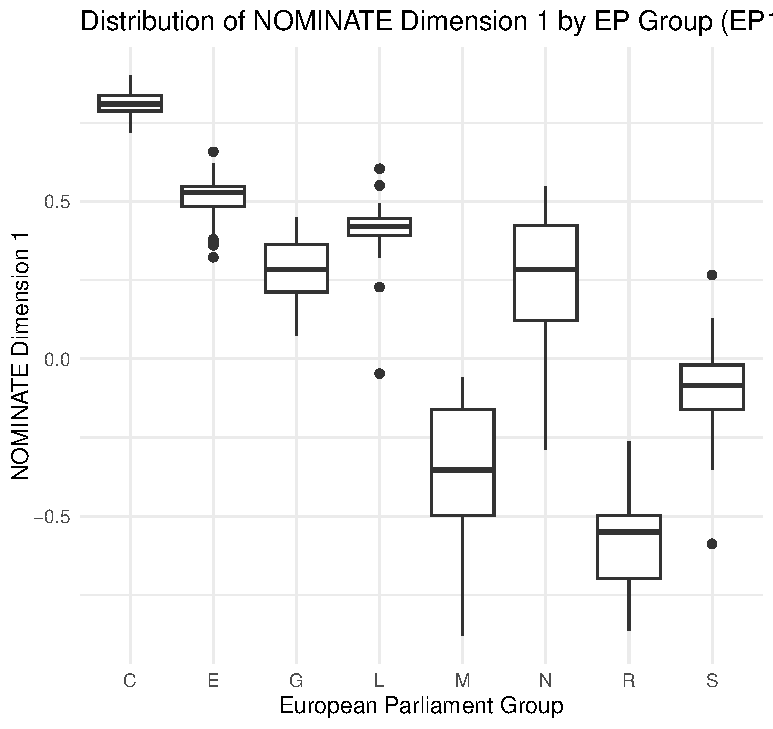
\includepdf[pages=-, scale=0.8]{plot1.pdf}
	\item Make a histogram using \texttt{geom\_col()} detailing the number of official members using the 12-level religious classification (\texttt{TRAD12}) distinguishing between the 6-level religious classification (\texttt{TRAD6}) in 2022. Hint: Use \texttt{facet()} for \texttt{TRAD6}, with \texttt{TRAD12} on the x-axis in addition to group/fill with the \texttt{position="dodge"}.
	\lstinputlisting[firstline=64,lastline=74]{PS02_RS.R}
	\includepdf[pages=-, scale=0.9]{plot2.pdf}
	\item Display the distribution of yearly income (\texttt{INCOME}) in 2022 for congregations in each region (\texttt{GDREGION}) using ridge plots.
	\lstinputlisting[firstline=76,lastline=94]{PS02_RS.R}
	\includepdf[pages=-, scale=0.9]{plot3.pdf}
	\item Create a boxplot of the number of official members per congregation in 2022 by religious classification (\texttt{TRAD6}) and region (\texttt{GDREGION}). Hint: Use \texttt{facet()} for \texttt{GDREGION}.
		\lstinputlisting[firstline=96,lastline=112]{PS02_RS.R}
	\includepdf[pages=-, scale=0.9]{plot4.pdf}

\end{enumerate}


\end{document}
